% Options for packages loaded elsewhere
\PassOptionsToPackage{unicode}{hyperref}
\PassOptionsToPackage{hyphens}{url}
%
\documentclass[
]{article}
\usepackage{lmodern}
\usepackage{amsmath}
\usepackage{ifxetex,ifluatex}
\ifnum 0\ifxetex 1\fi\ifluatex 1\fi=0 % if pdftex
  \usepackage[T1]{fontenc}
  \usepackage[utf8]{inputenc}
  \usepackage{textcomp} % provide euro and other symbols
  \usepackage{amssymb}
\else % if luatex or xetex
  \usepackage{unicode-math}
  \defaultfontfeatures{Scale=MatchLowercase}
  \defaultfontfeatures[\rmfamily]{Ligatures=TeX,Scale=1}
\fi
% Use upquote if available, for straight quotes in verbatim environments
\IfFileExists{upquote.sty}{\usepackage{upquote}}{}
\IfFileExists{microtype.sty}{% use microtype if available
  \usepackage[]{microtype}
  \UseMicrotypeSet[protrusion]{basicmath} % disable protrusion for tt fonts
}{}
\makeatletter
\@ifundefined{KOMAClassName}{% if non-KOMA class
  \IfFileExists{parskip.sty}{%
    \usepackage{parskip}
  }{% else
    \setlength{\parindent}{0pt}
    \setlength{\parskip}{6pt plus 2pt minus 1pt}}
}{% if KOMA class
  \KOMAoptions{parskip=half}}
\makeatother
\usepackage{xcolor}
\IfFileExists{xurl.sty}{\usepackage{xurl}}{} % add URL line breaks if available
\IfFileExists{bookmark.sty}{\usepackage{bookmark}}{\usepackage{hyperref}}
\hypersetup{
  pdftitle={R-Bootcamp Report},
  pdfauthor={Bernardo Freire Barboza da Cruz \& Leonid Gavrilyuk},
  hidelinks,
  pdfcreator={LaTeX via pandoc}}
\urlstyle{same} % disable monospaced font for URLs
\usepackage[margin=1in]{geometry}
\usepackage{graphicx}
\makeatletter
\def\maxwidth{\ifdim\Gin@nat@width>\linewidth\linewidth\else\Gin@nat@width\fi}
\def\maxheight{\ifdim\Gin@nat@height>\textheight\textheight\else\Gin@nat@height\fi}
\makeatother
% Scale images if necessary, so that they will not overflow the page
% margins by default, and it is still possible to overwrite the defaults
% using explicit options in \includegraphics[width, height, ...]{}
\setkeys{Gin}{width=\maxwidth,height=\maxheight,keepaspectratio}
% Set default figure placement to htbp
\makeatletter
\def\fps@figure{htbp}
\makeatother
\setlength{\emergencystretch}{3em} % prevent overfull lines
\providecommand{\tightlist}{%
  \setlength{\itemsep}{0pt}\setlength{\parskip}{0pt}}
\setcounter{secnumdepth}{5}
\ifluatex
  \usepackage{selnolig}  % disable illegal ligatures
\fi

\title{R-Bootcamp Report}
\author{Bernardo Freire Barboza da Cruz \& Leonid Gavrilyuk}
\date{03 February, 2022}

\begin{document}
\maketitle

{
\setcounter{tocdepth}{2}
\tableofcontents
}
\pagebreak

\hypertarget{introduction}{%
\section{Introduction}\label{introduction}}

Describe the use case\ldots.

\begin{enumerate}
\def\labelenumi{\arabic{enumi}.}
\tightlist
\item
  Most active districts\\
\item
  Party dynamics 2006-2018\\
\item
  Activity of genders (e.g.~women are active voters)\\
\item
  Activity of age groups\\
\item
  Relationships between education and activity.\\
\item
  Relationships between income and activity.
\end{enumerate}

\pagebreak

\hypertarget{extract-and-transform}{%
\section{Extract and Transform}\label{extract-and-transform}}

\hypertarget{data-import}{%
\subsection{Data Import}\label{data-import}}

The data is imported from
\emph{\href{https://data.stadt-zuerich.ch/}{Stadt Zürich Open Data}}.

\hypertarget{exploration-wealth-and-income-data}{%
\subsubsection{Exploration: Wealth and Income
data}\label{exploration-wealth-and-income-data}}

\hypertarget{wealth-data}{%
\paragraph{Wealth Data}\label{wealth-data}}

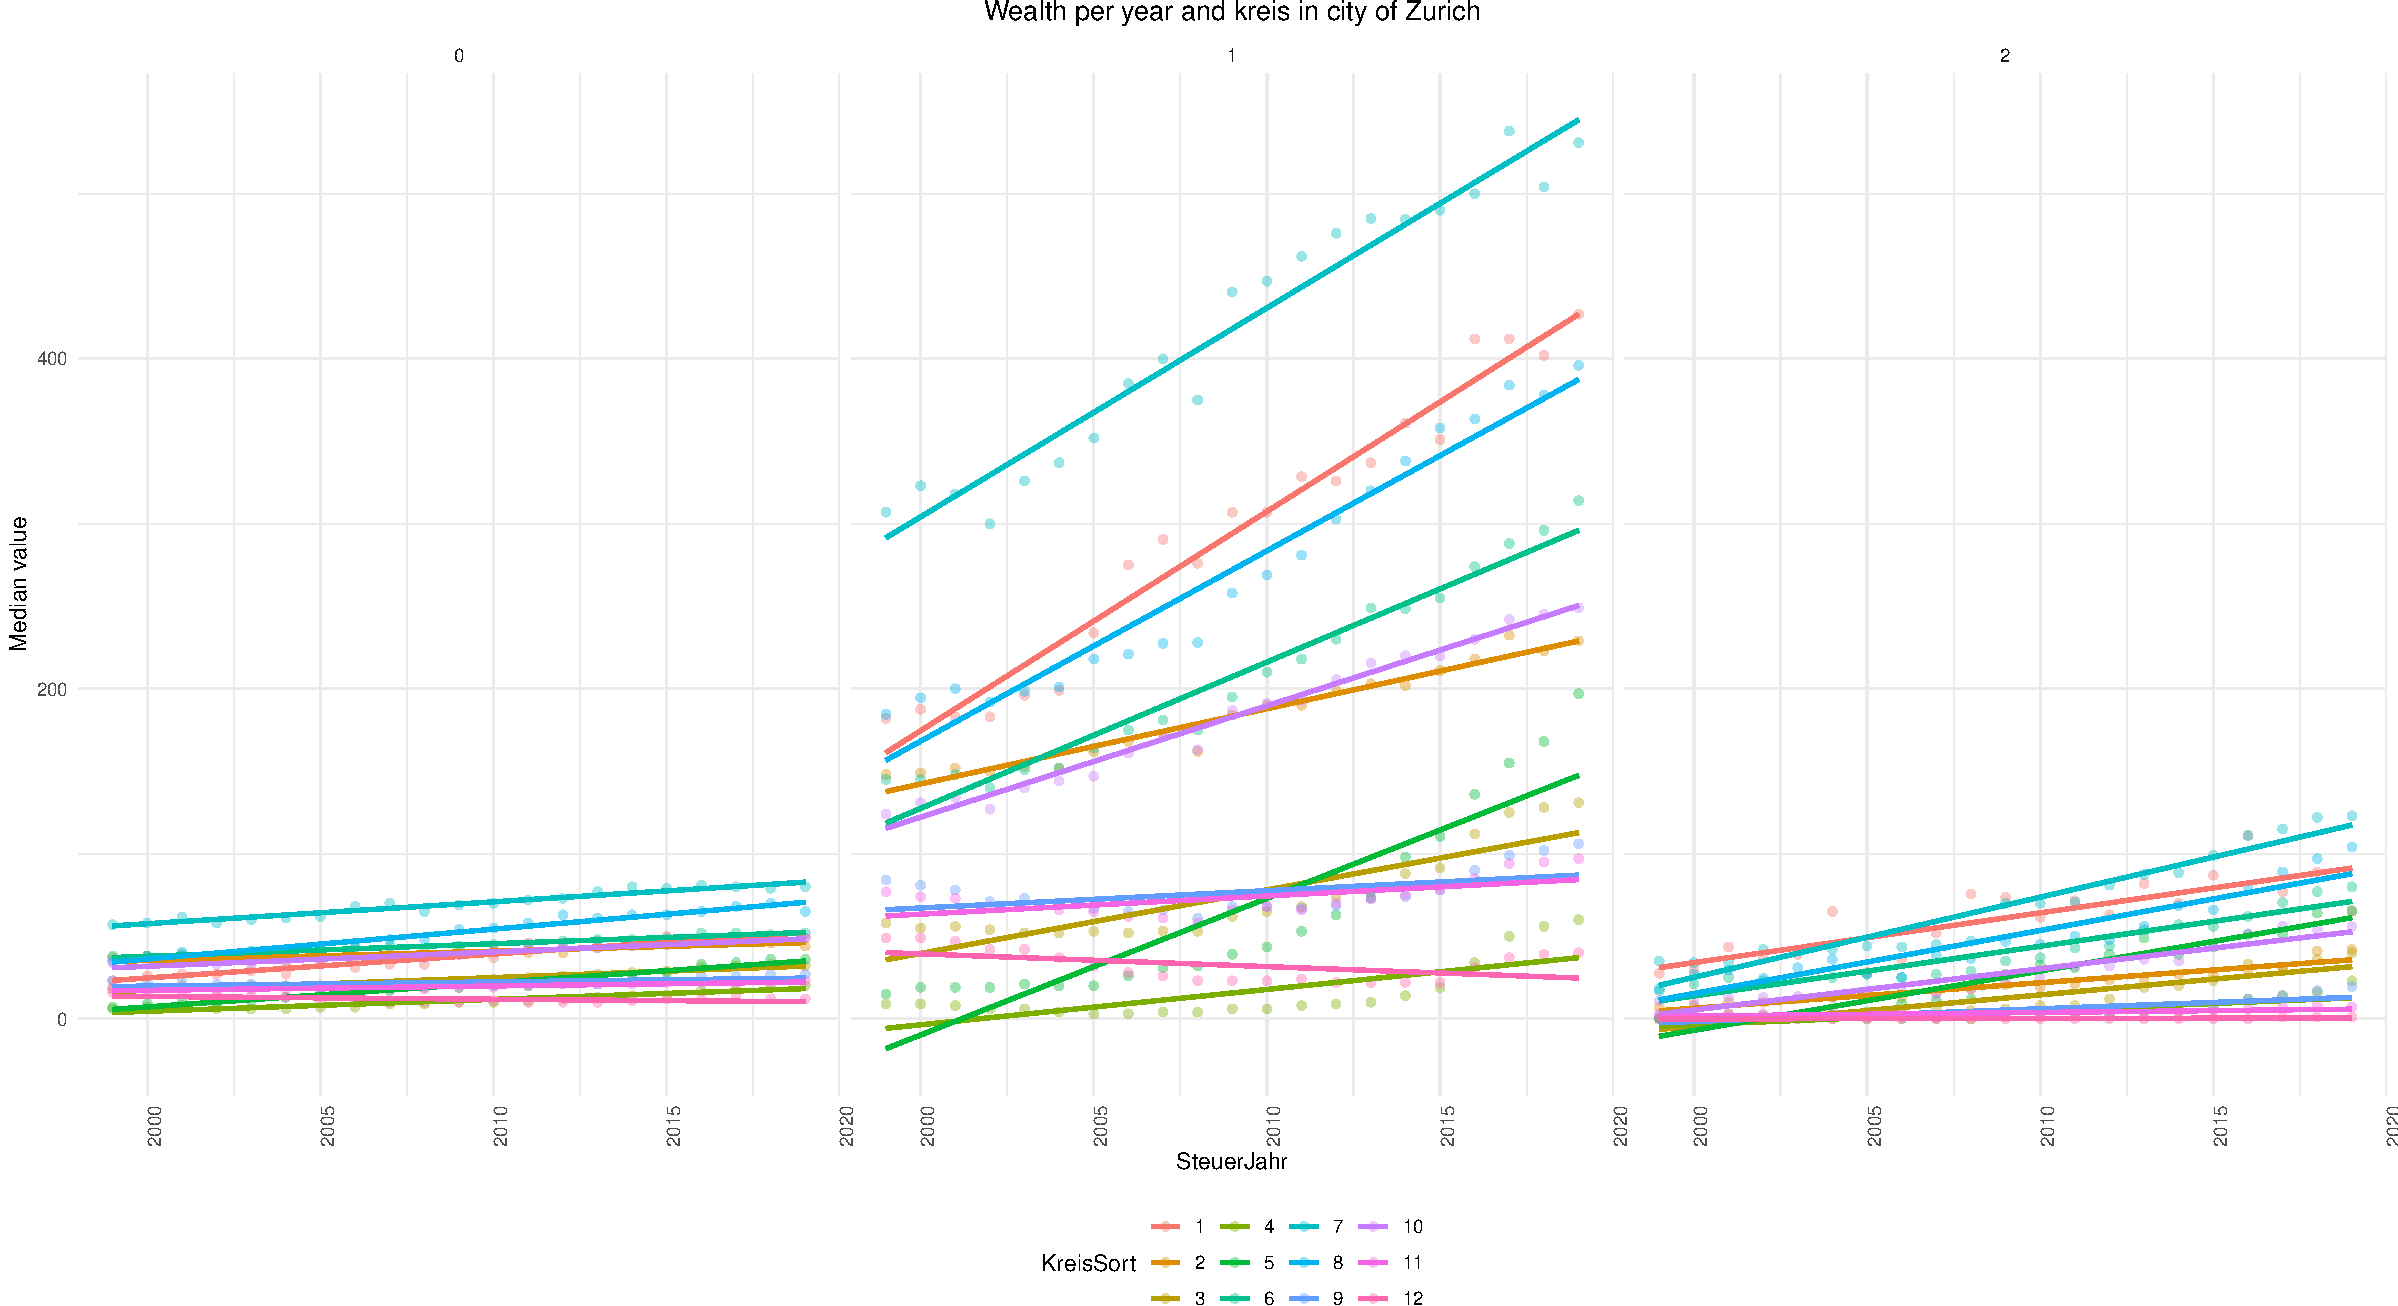
\includegraphics{report_files/figure-latex/plot_wealth-1.pdf}

\hypertarget{income}{%
\paragraph{Income}\label{income}}

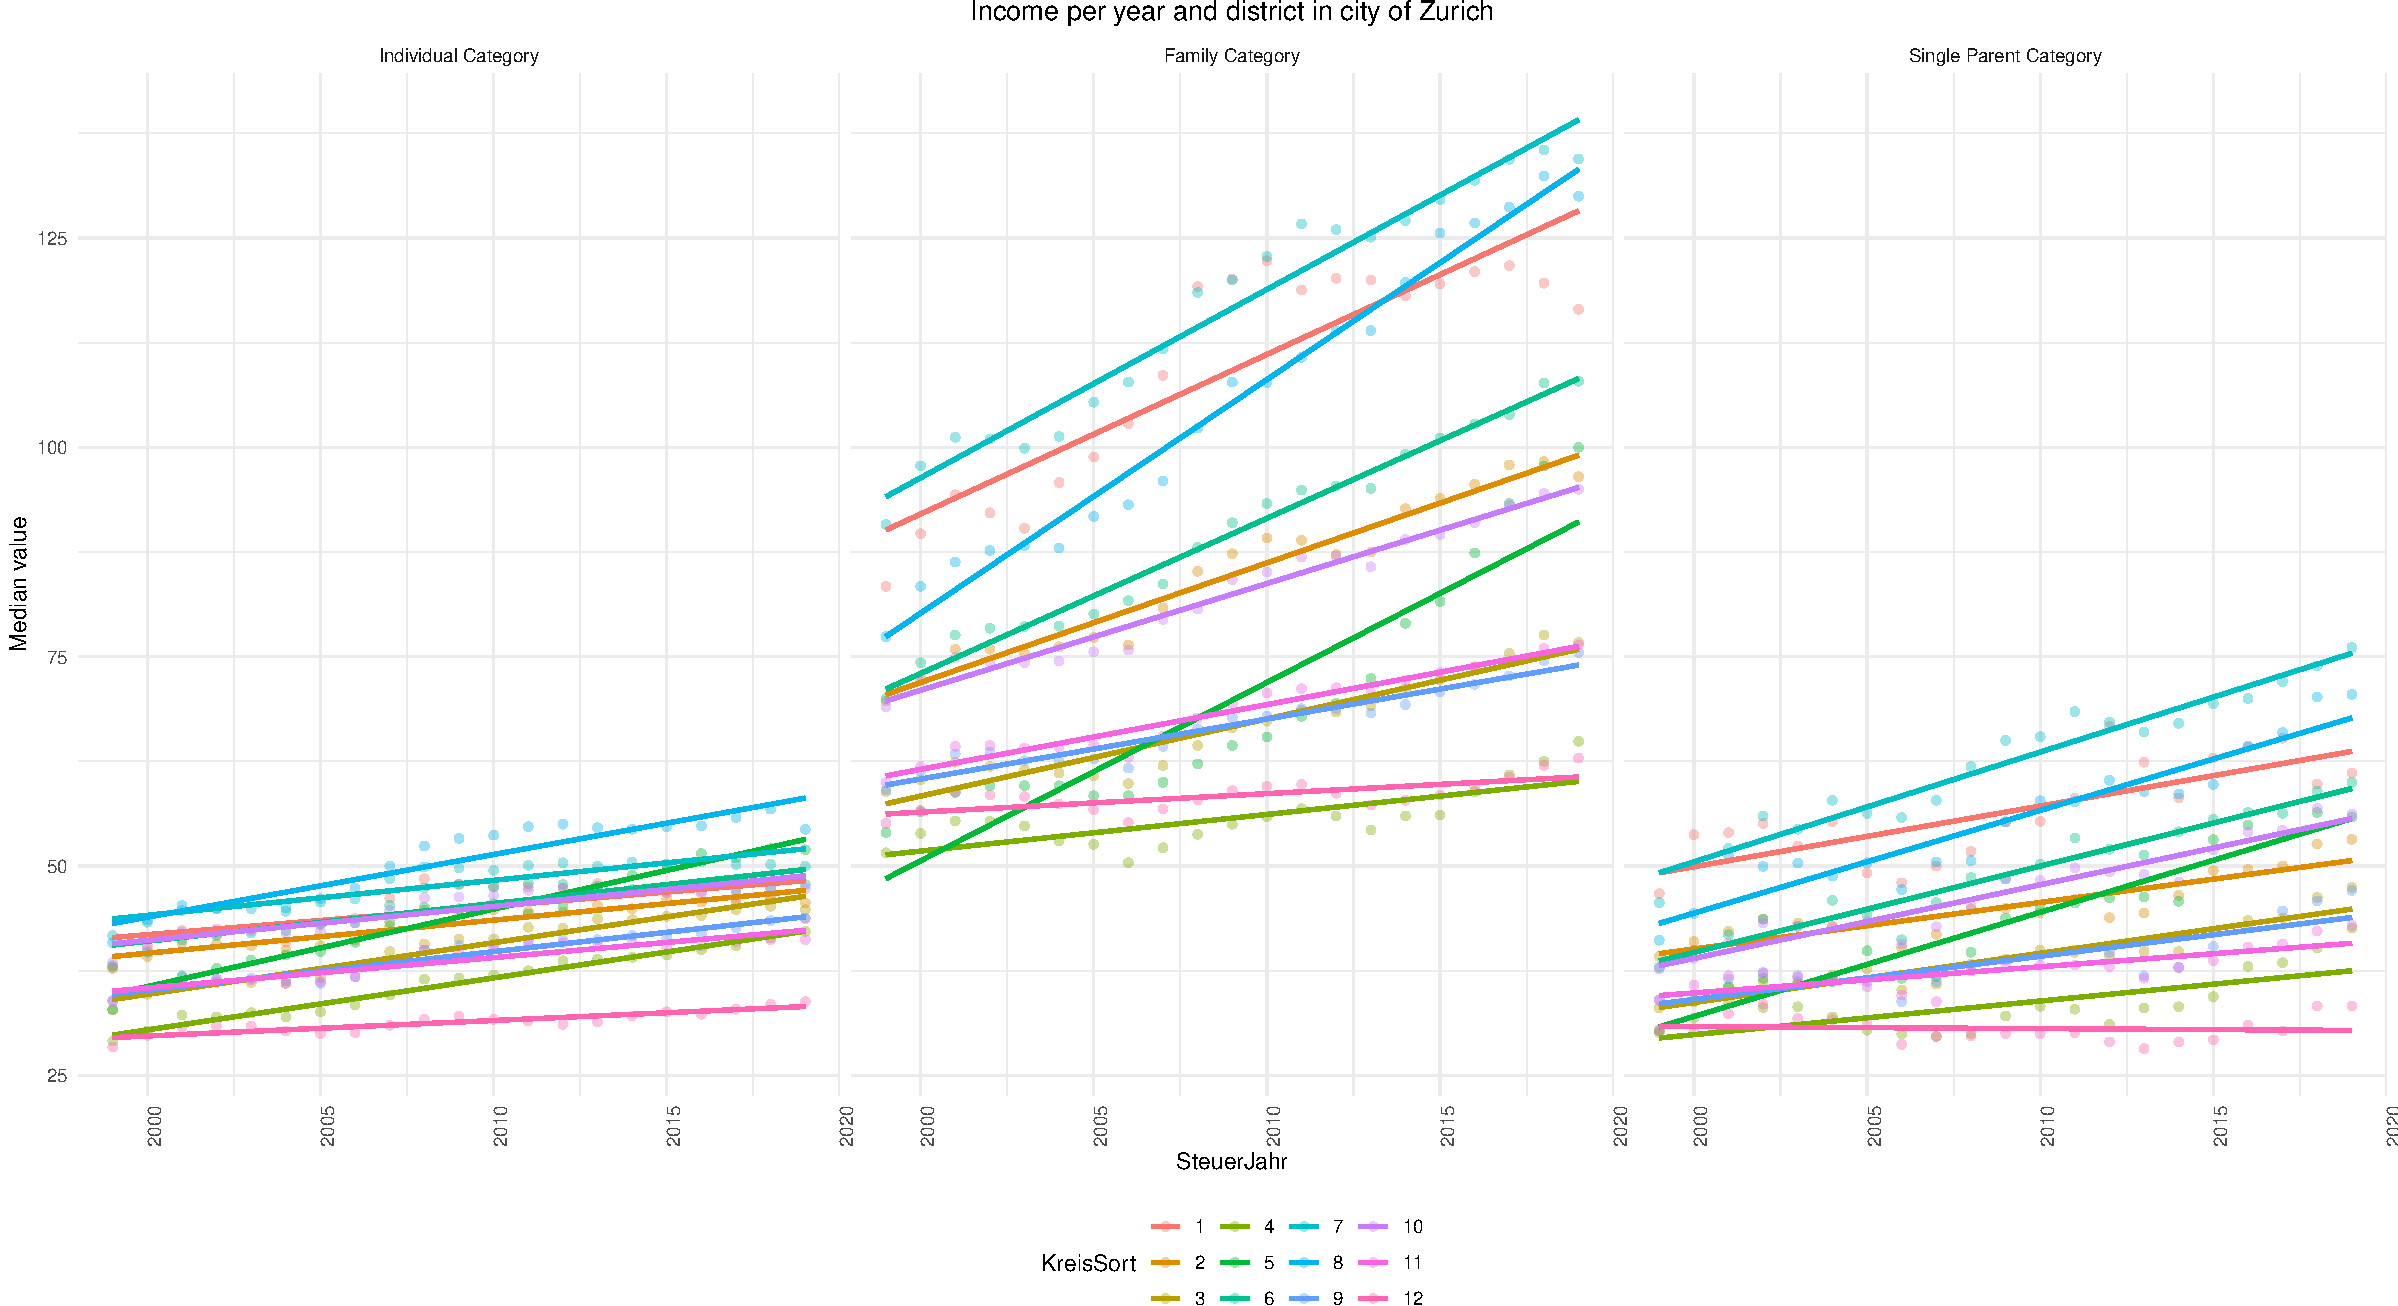
\includegraphics{report_files/figure-latex/plot_income-1.pdf}

\hypertarget{exploration-education}{%
\subsubsection{Exploration: Education}\label{exploration-education}}

\hypertarget{preproces-data}{%
\paragraph{Preproces Data}\label{preproces-data}}

The encoding of the column \texttt{RaumSort} consists of the Kreis and
further local details. The last digit describes neighborhood of each
Kreis. It means:

\begin{itemize}
\tightlist
\item
  Two digits: The first digit describes the Kreis and the second the
  neighborhood
\item
  Three digits: The first \emph{two} digits describes the Kreis and the
  third the neighborhood
\end{itemize}

Add a new column to dataset for Kreis and neighborhood.

\hypertarget{data-exploration-visualization}{%
\subsection{Data Exploration \&
Visualization}\label{data-exploration-visualization}}

\hypertarget{merging-data}{%
\subsection{Merging Data}\label{merging-data}}

\hypertarget{data-visualization}{%
\subsection{Data Visualization}\label{data-visualization}}

\hypertarget{fit-model}{%
\subsection{Fit Model}\label{fit-model}}

\hypertarget{chapter-of-choice-tbd}{%
\subsection{Chapter of Choice TBD}\label{chapter-of-choice-tbd}}

\hypertarget{references}{%
\section{References}\label{references}}

\end{document}
